\documentclass[13pt]{article}
\usepackage{graphicx}

%opening
\title{Mis apuntes de las clases de Git y Github}
\author{Jhamil Arnez Hidalgo}
\date{Última actualización: \today}

\begin{document}

\maketitle


\section{¿Qué es Git?}
Git es es un sistema de control de versiones distribuido que permite a los desarrolladores llevar un registro de los cambios en sus archivos y coordinar el trabajo en proyectos de software de manera eficiente.\\

Distribuido quiere decir que no depende de un único sitio en específico para almacenar su código. Existen muchos controladores de versiones, pero no todos son distribuidos, eso significa que por ejemplo si el servidor donde tienen almacenado el código llega a reventar, entonces perderían todo el código.\\

En cambio, un sistema distribuido permite tener a todos los colaboradores una copia del proyecto en sus propios equipos, y en caso de que el servidor principal reventase, el proyecto seguiría existiendo en las máquinas personales de los desarrolladores y se podría recuperar.

\section{Comandos de Git}

\subsection{Git Init}
Para empezar a usar git, primero se necesita un repositorio local, es decir una carpeta, sobre la cual git va a ir controlando y guardando sus versiones y revisando sus cambios.\\

Una vez creada la carpeta, desde la terminal hay que posicionarse sobre esa carpeta (en bash con cd ~/directorio).\\

Una vez hecho esto en la terminal se va a escribir, \textbf{git init} y esto automáticamente creará una carpeta oculta llamada ".git" en la carpeta.\\
\begin{figure}[h!]
	\centering
	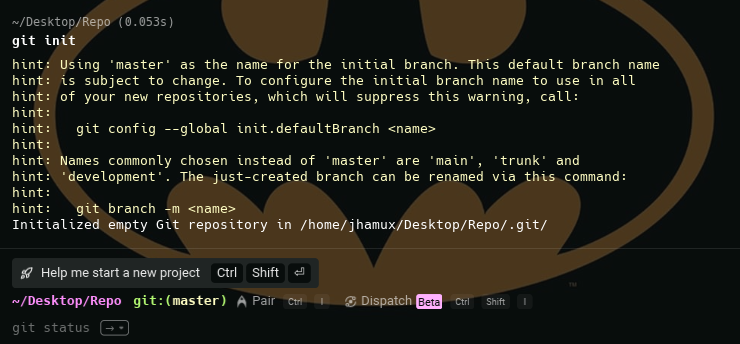
\includegraphics[scale = 0.6]{Images/gitinit.png}
	\caption{Git Init ejecutado en la terminal}
	
	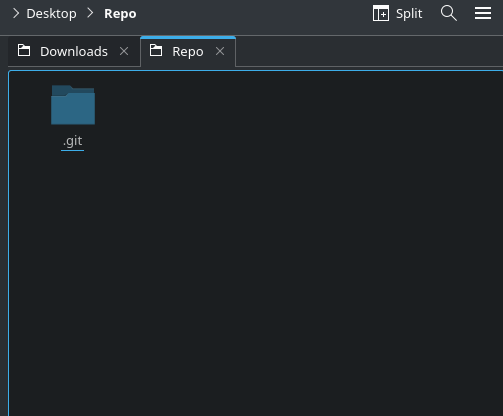
\includegraphics[scale = 0.6]{Images/dotgit.png}
	\caption{Carpeta Oculta .git en el repositorio}
\end{figure}

\subsection{Git Add y Git Commit}
Ahora que git está monitoreando el repositorio podemos crear un fichero de lo que gustemos y git lo detectará, pero no lo guardará automáticamente, es importante entender los 3 estados en los que puede estar un fichero en un repositorio con git.\\
\begin{enumerate}
	\item \textbf{modified:} El archivo tiene cambios pero aún no fueron marcados para ser confirmados, se encuentra en el directorio de trabajo.
	\item \textbf{staged:} Son los archivos que fueron modificados y confirmados para guardarse en el repositorio local, se encuentran en un área temporal transitoria.
	\item \textbf{commited:} El archivo se encuentra grabado en el repositorio local.
\end{enumerate}

Cuando creamos un archivo nuevo, git no lo reconocerá automáticamente, aparecerá como "untracked" para que git empiece a hacerle seguimiento hay que ejecutar el comando: \textbf{git add nombre-del-archivo}, y así pasará al estado de \textbf{staged}.\\

Una vez que todos los archivos se encuentren en el estado staged, estaŕan listos para que se les pueda realizar un commit, básicamente les estamos sacando una foto en el momento actual a todos los archivos, guardando el momento. Esto se hace con el comando \textbf{git commit}, este comando nos abrirá un editor de código para colocar un nombre al commit, una vez colocado el nombre el commit ya queda realizado.

\subsection{Git Log y Git Status}
Estos comandos son para observar el estado de tus commits y de tu repositorio respectivamente.\\

El comando \textbf{git log}, nos muestra todos los commits existentes en una lista, donde nos muestra el nombre de los commits, la hora y fecha de creación, el código hash de los commits, y el autor de este mismo.\\
También existen diferentes formas de visualizarlo, una bastante práctica es escribir el comando: \textbf{git log --oneline} donde te muestra todos los commits cada uno en una línea, haciendo más práctico su visualización.

\begin{figure}[!h]
	\centering
	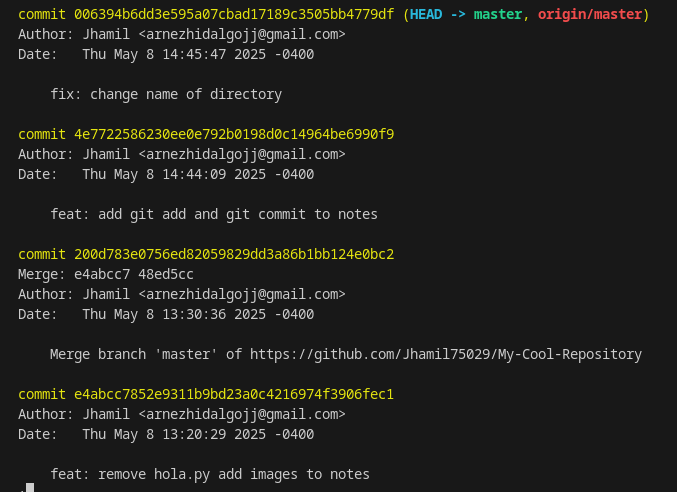
\includegraphics[scale = 0.4]{Images/gitlog1.png}
	\caption {\small Git Log en la consola}
	
	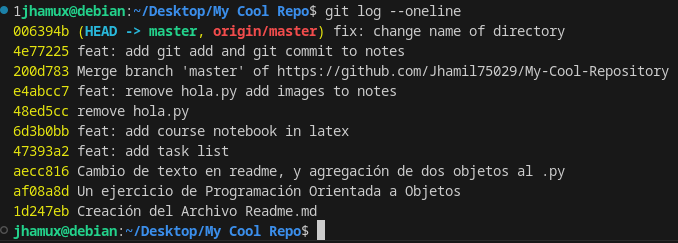
\includegraphics[scale = 0.4]{Images/gitlog2.png}
	\caption {\small Git Log in one line en la consola}
\end{figure}

El comando \textbf{git status}, nos muestra la lista de todos los archivos que estén en estado staged, modified, y si es nuevo, untracked. Así como también nos muestra si no hay novedades en el repositorio.\\

\begin{figure}[!h]
	\centering
	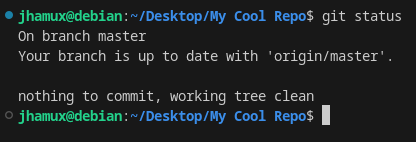
\includegraphics[scale = 0.7]{Images/gitstatus.png}
	\caption {\small Git Status en la consola}
\end{figure}

\section{Alias}
Los alias son formas de nombrar una serie de comandos en una sola palabra, como si se tratase de un atajo de teclado, nosotros podemos crear un alias para una sucesión de códigos de git larga y para ejecutarla solo redactando una palabra.\\

\begin{figure}[!h]
	\centering
	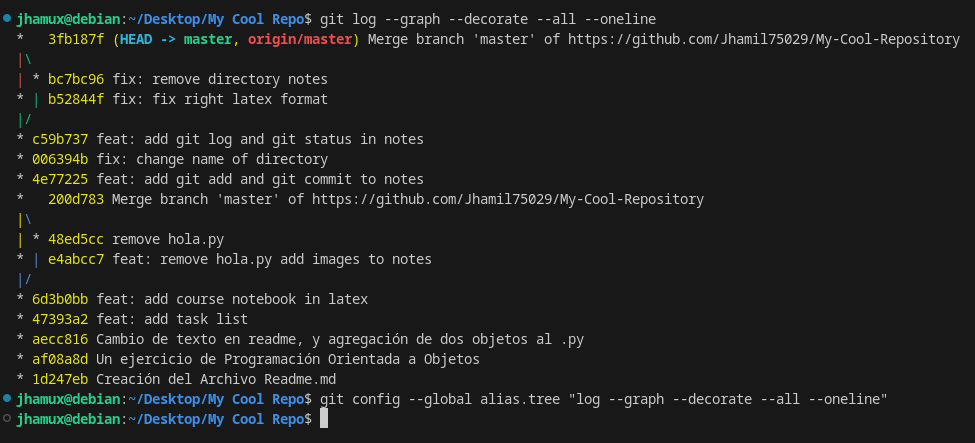
\includegraphics[scale = 0.6]{Images/alias1.png}
	\caption {\small Creamos un alias para git log graph decorate all y oneline}
\end{figure}


\end{document}
